\section{WC 28/4/25}

\subsection*{Overview:}
This week was the final leadup to my L6 Mock exams, Having prepared for this in my timeline/plan (and having been working ahead of my plan once again these last few weeks) I had no tasks to complete this week and so just spent some spare moments 'tying up loose ends' and making small improvements.
\subsection*{Achievements, Thoughts and Ideas:}


I had observed a couple of visual bugs within my app in which specific UI elements (such as the mini graph view in the dashboard) would constantly resize and shrink as the display size was on the boundary of my small / medium screen size (see image and video right). Whilst I didn’t think this would be an common it seems that on some android tablets this is a fairly common resolution and required a solution. I researched the cause of this online by searching a number of forum threads (dating back up to 15 years!) and this seems to be a common issue faced by frontend developers. Whilst I haven't yet found a perfect solution I've pushed a quick patch (which removes the flashing scroll bars but not the overflowing elements)
\begin{figure}[H]
    \centering
    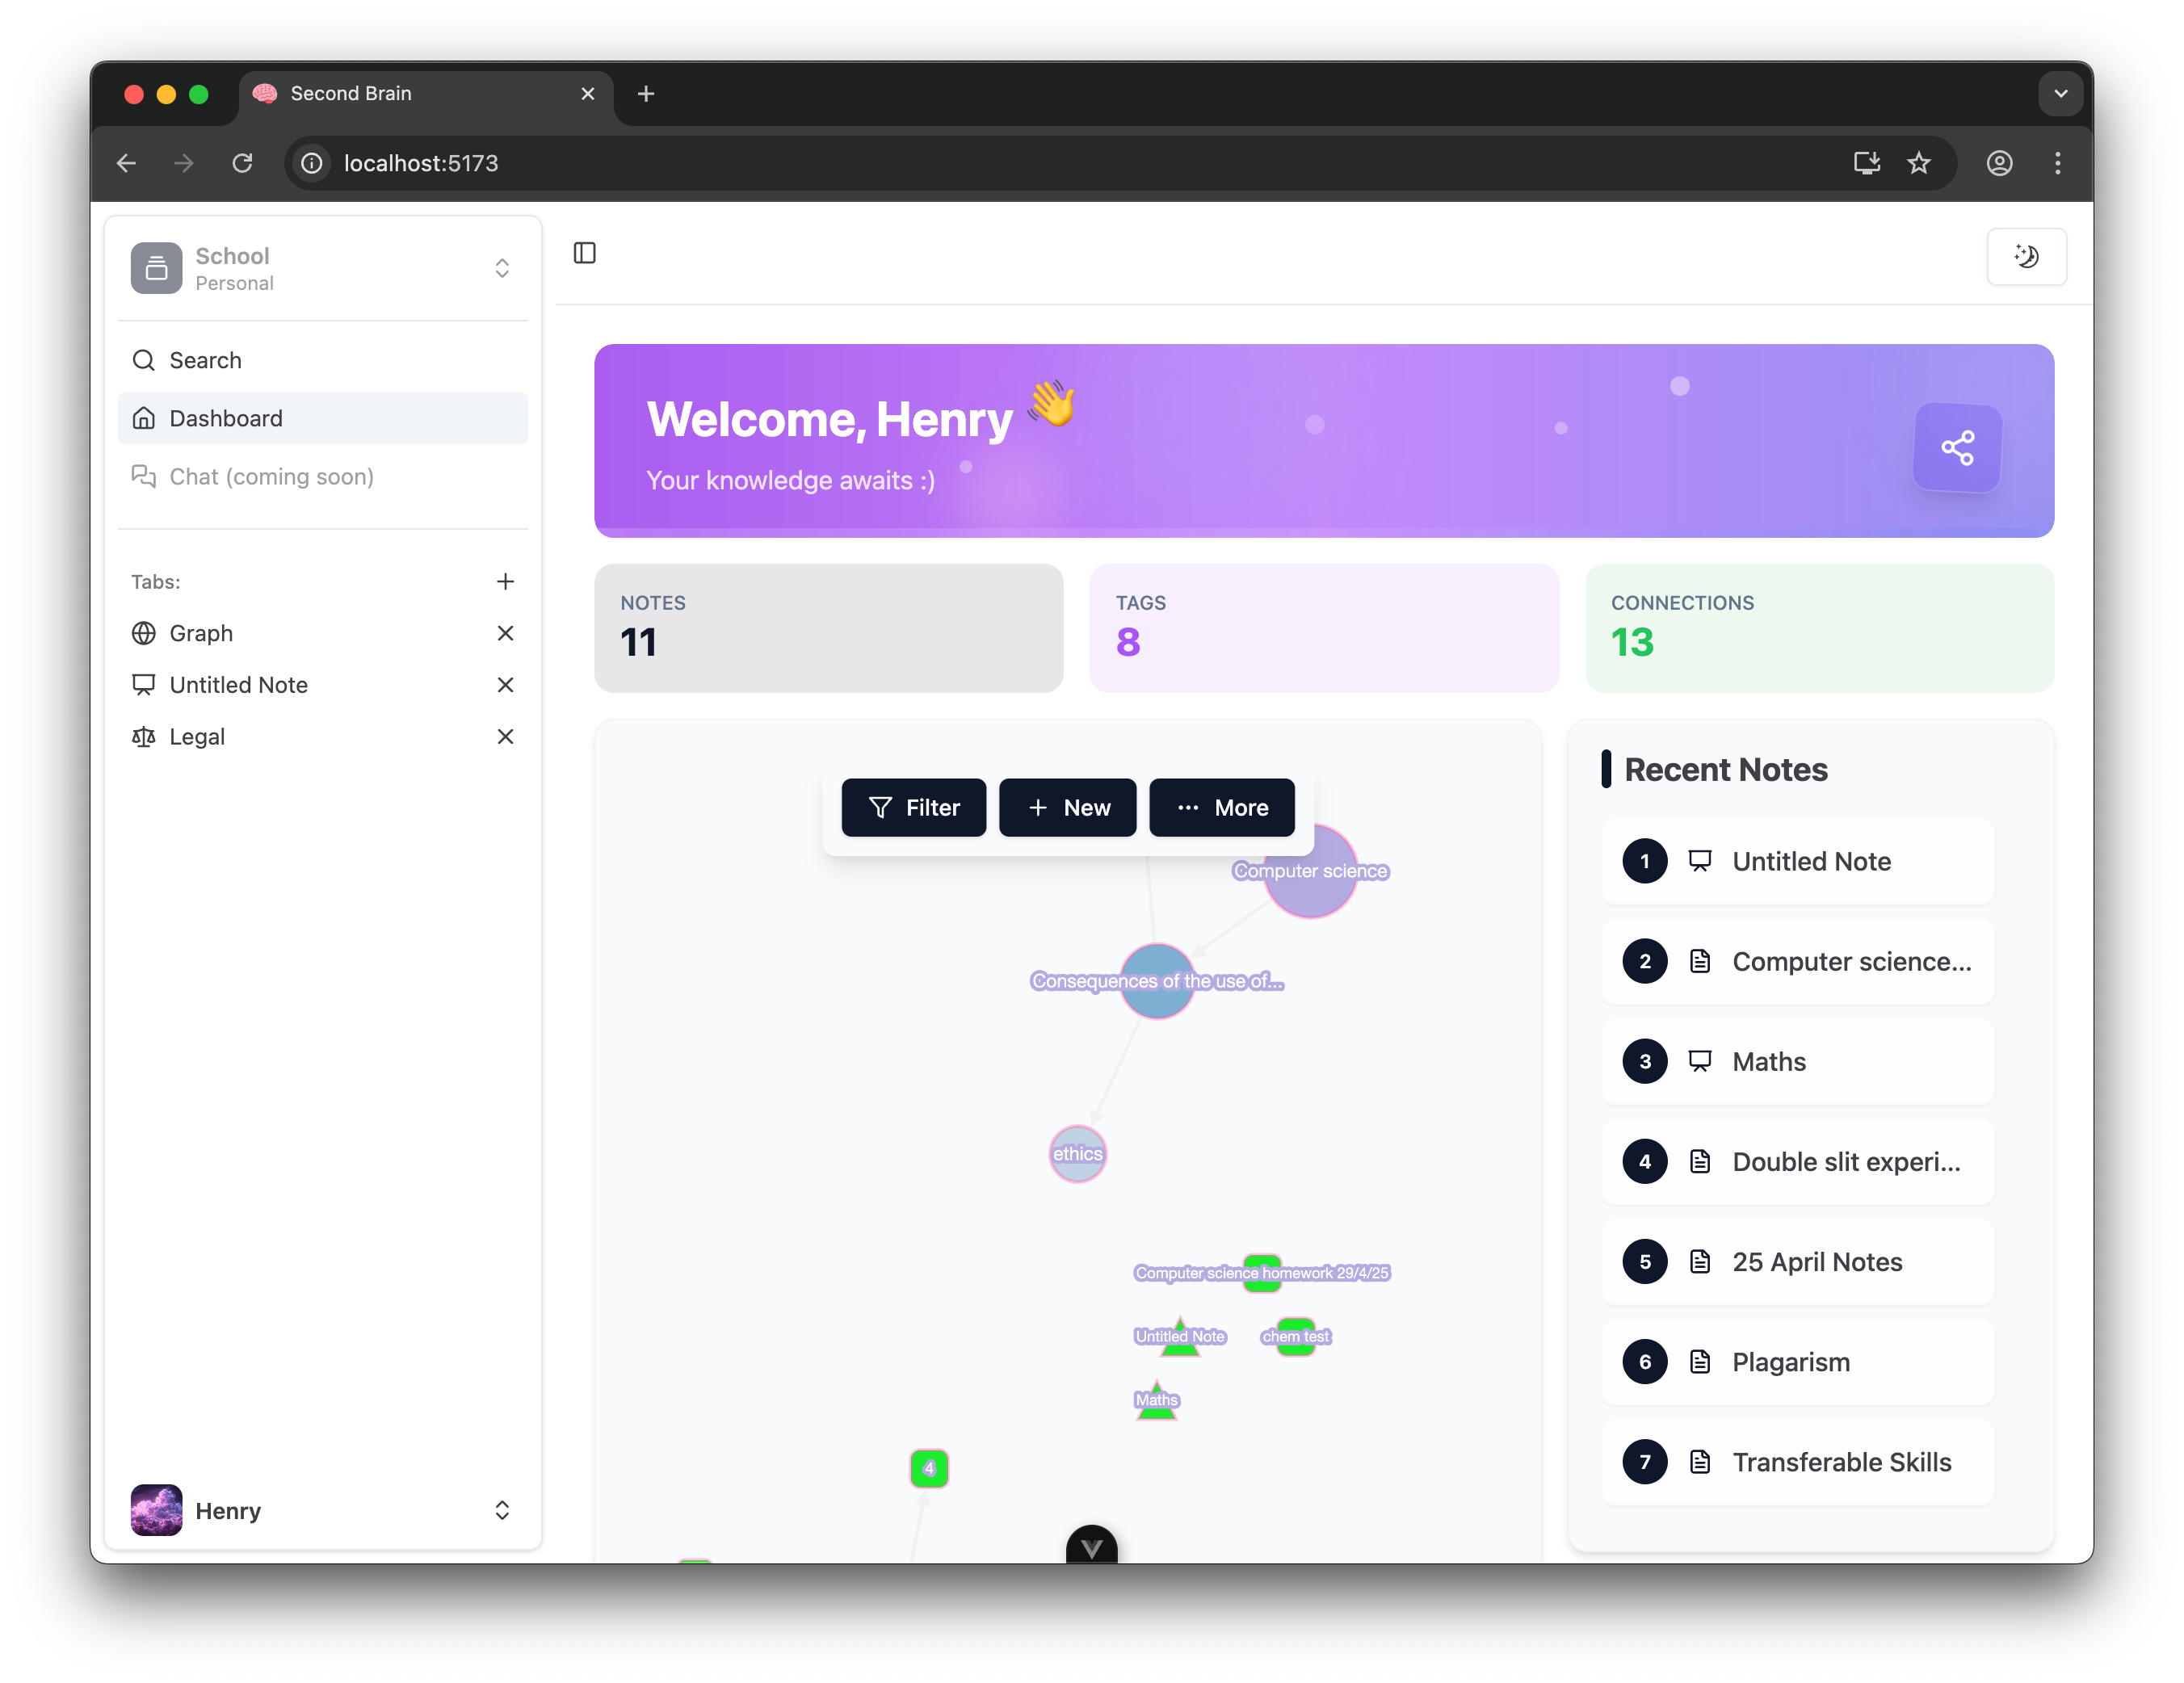
\includegraphics[width=0.8\linewidth]{Diary/27_WC_28-4-25/media/noFlash.png}
    \caption{Scrollbar flashing issue on small displays solved}
    \label{fig:resizing_issue}
\end{figure}

I built a popup menu which allows user to select the dashboard shortcuts which enables maximal productivity through customisability. This required some new backend database development (to allow for a very customisable yet restricted data input to ensure users can't set an impossible shortcut and render their system unstable)
\begin{figure}[H]
    \centering
    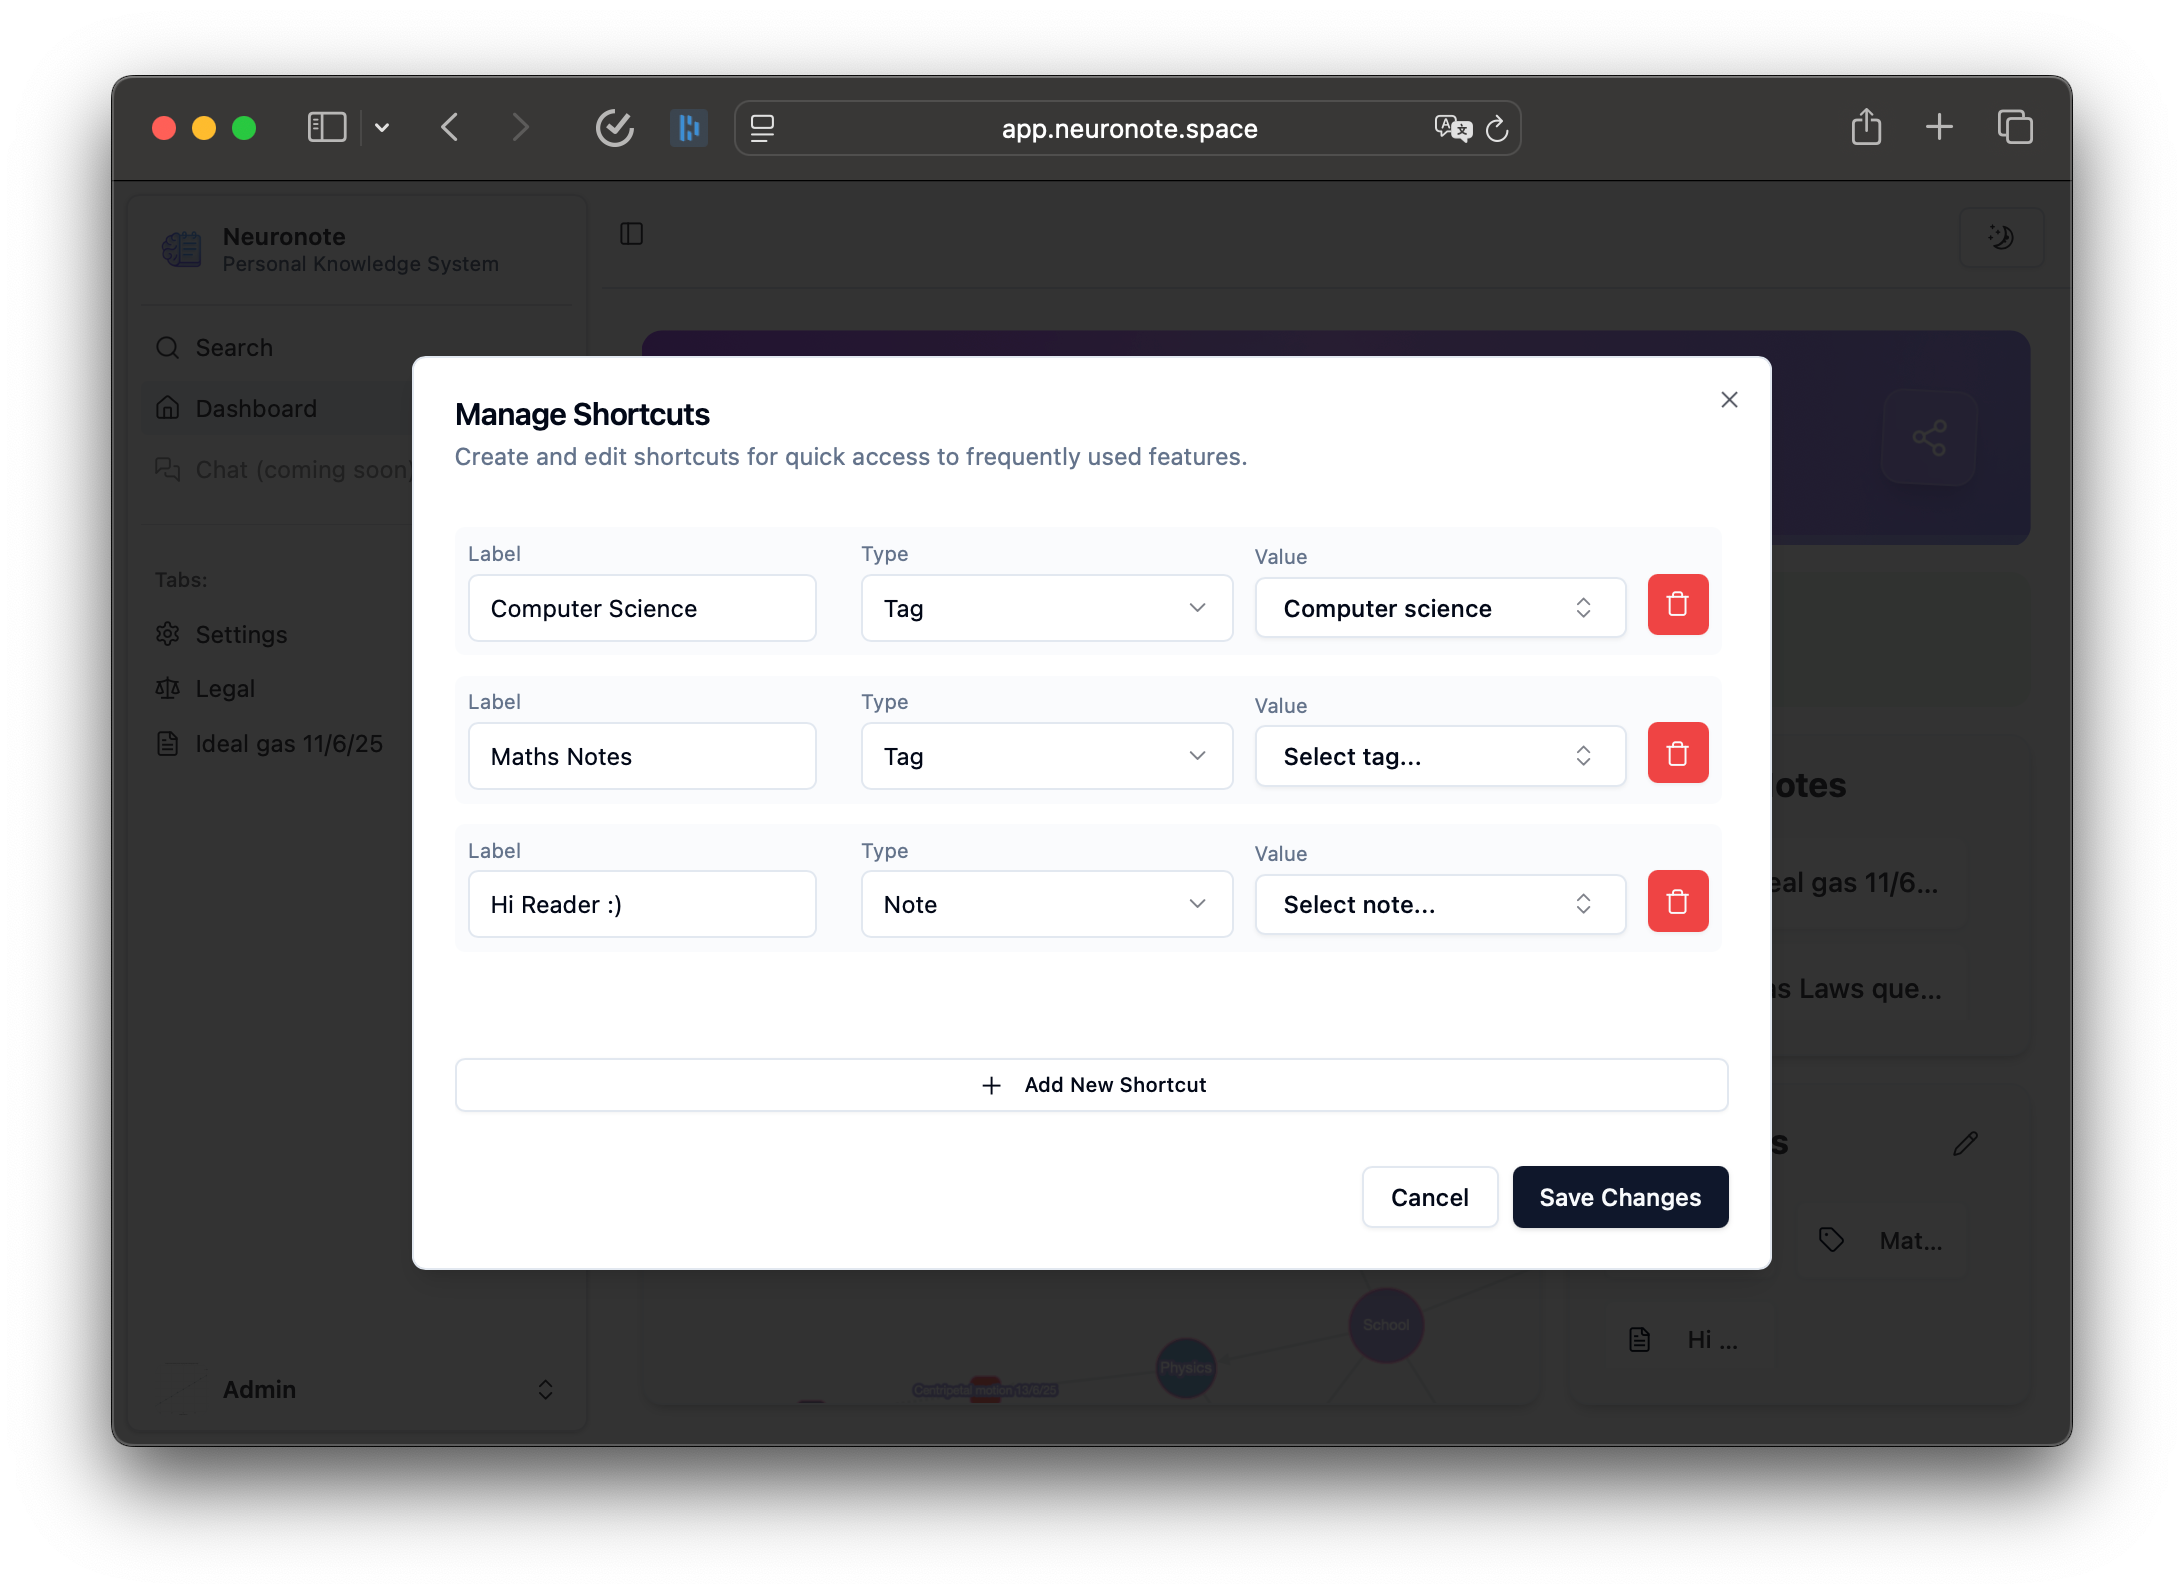
\includegraphics[width=0.8\linewidth]{Diary/27_WC_28-4-25/media/shortcutPanel.png}
    \caption{New shortcuts menu}
    \label{fig:shortcuts_menu}
\end{figure}

As mentioned last week I switched the order of the final weeks in April around so that I could spend this week on the more creative task of deciding on a colour theme and branding for my project.

Approaching colour themes of the project:
So far in my EPQ journey I have looked into colour theory and the meanings people often associate to colour in addition to the impact colour can have on accessibility for a variety of users and fundamentally the impact it can have on our ability to learn content (which is the fundamental idea within my academic project). From the very start of the project I had liked the idea of a purple and blue hue to my software (these being my favourite colours) however I wanted to ensure I would avoid conformation bias in my decision and ensure the choice made was the right one for my users. To this extent I spent some time this week rereading my research on existing user interfaces to fundamentally ascertain what it was that made them successful and I came to this conclusion:

None of the products worked well because of their colours, and in fact, a number of complaints I had about existing provision stemmed from 'bold' design decisions being made that while visually appealing, drew away from the software's purpose: hiding key features, making text difficult to read and even being irritating on the eyes when used at night (lacking a good dark mode). From this I have drawn a very simple conclusion: that by keeping all of my interactive and text based elements a clean and 'sterile' monochrome colour I can ensure sufficient contrast and excellent readability across my platform. Additionally this gives me the future flexibility to allow users to add a custom hue to the background to match their tastes without reducing the benefits outlined above. Whilst my Ui will therefore remain largely monochromatic I am deciding to continue using purple/blue tones for my branding colours (as can be seen the prior few weeks)

Now to pick a name for my project:
To help generate some creative ideas I first turned to generative AI and got come ideas. Whilst none of these were a perfect fit it got me thinking about the various ideas I wanted to incorporate. Primarily these were the ideas of connection, clear signals this was a notetaking app, potential mythical links (furthering the academic connection). In the end I have settled on NeuroNote for my project name. it  signals idea about the brain, study and connections whilst also clearly identifying the software purpose (similar to OneNote or Evernote) I decided that as a new to the industry software this was important to raise awareness and prevent users being turned away / being confused by a more abstract name concept.


I have updated my webapp with this finalised branding:
\begin{figure}[H]
    \centering
    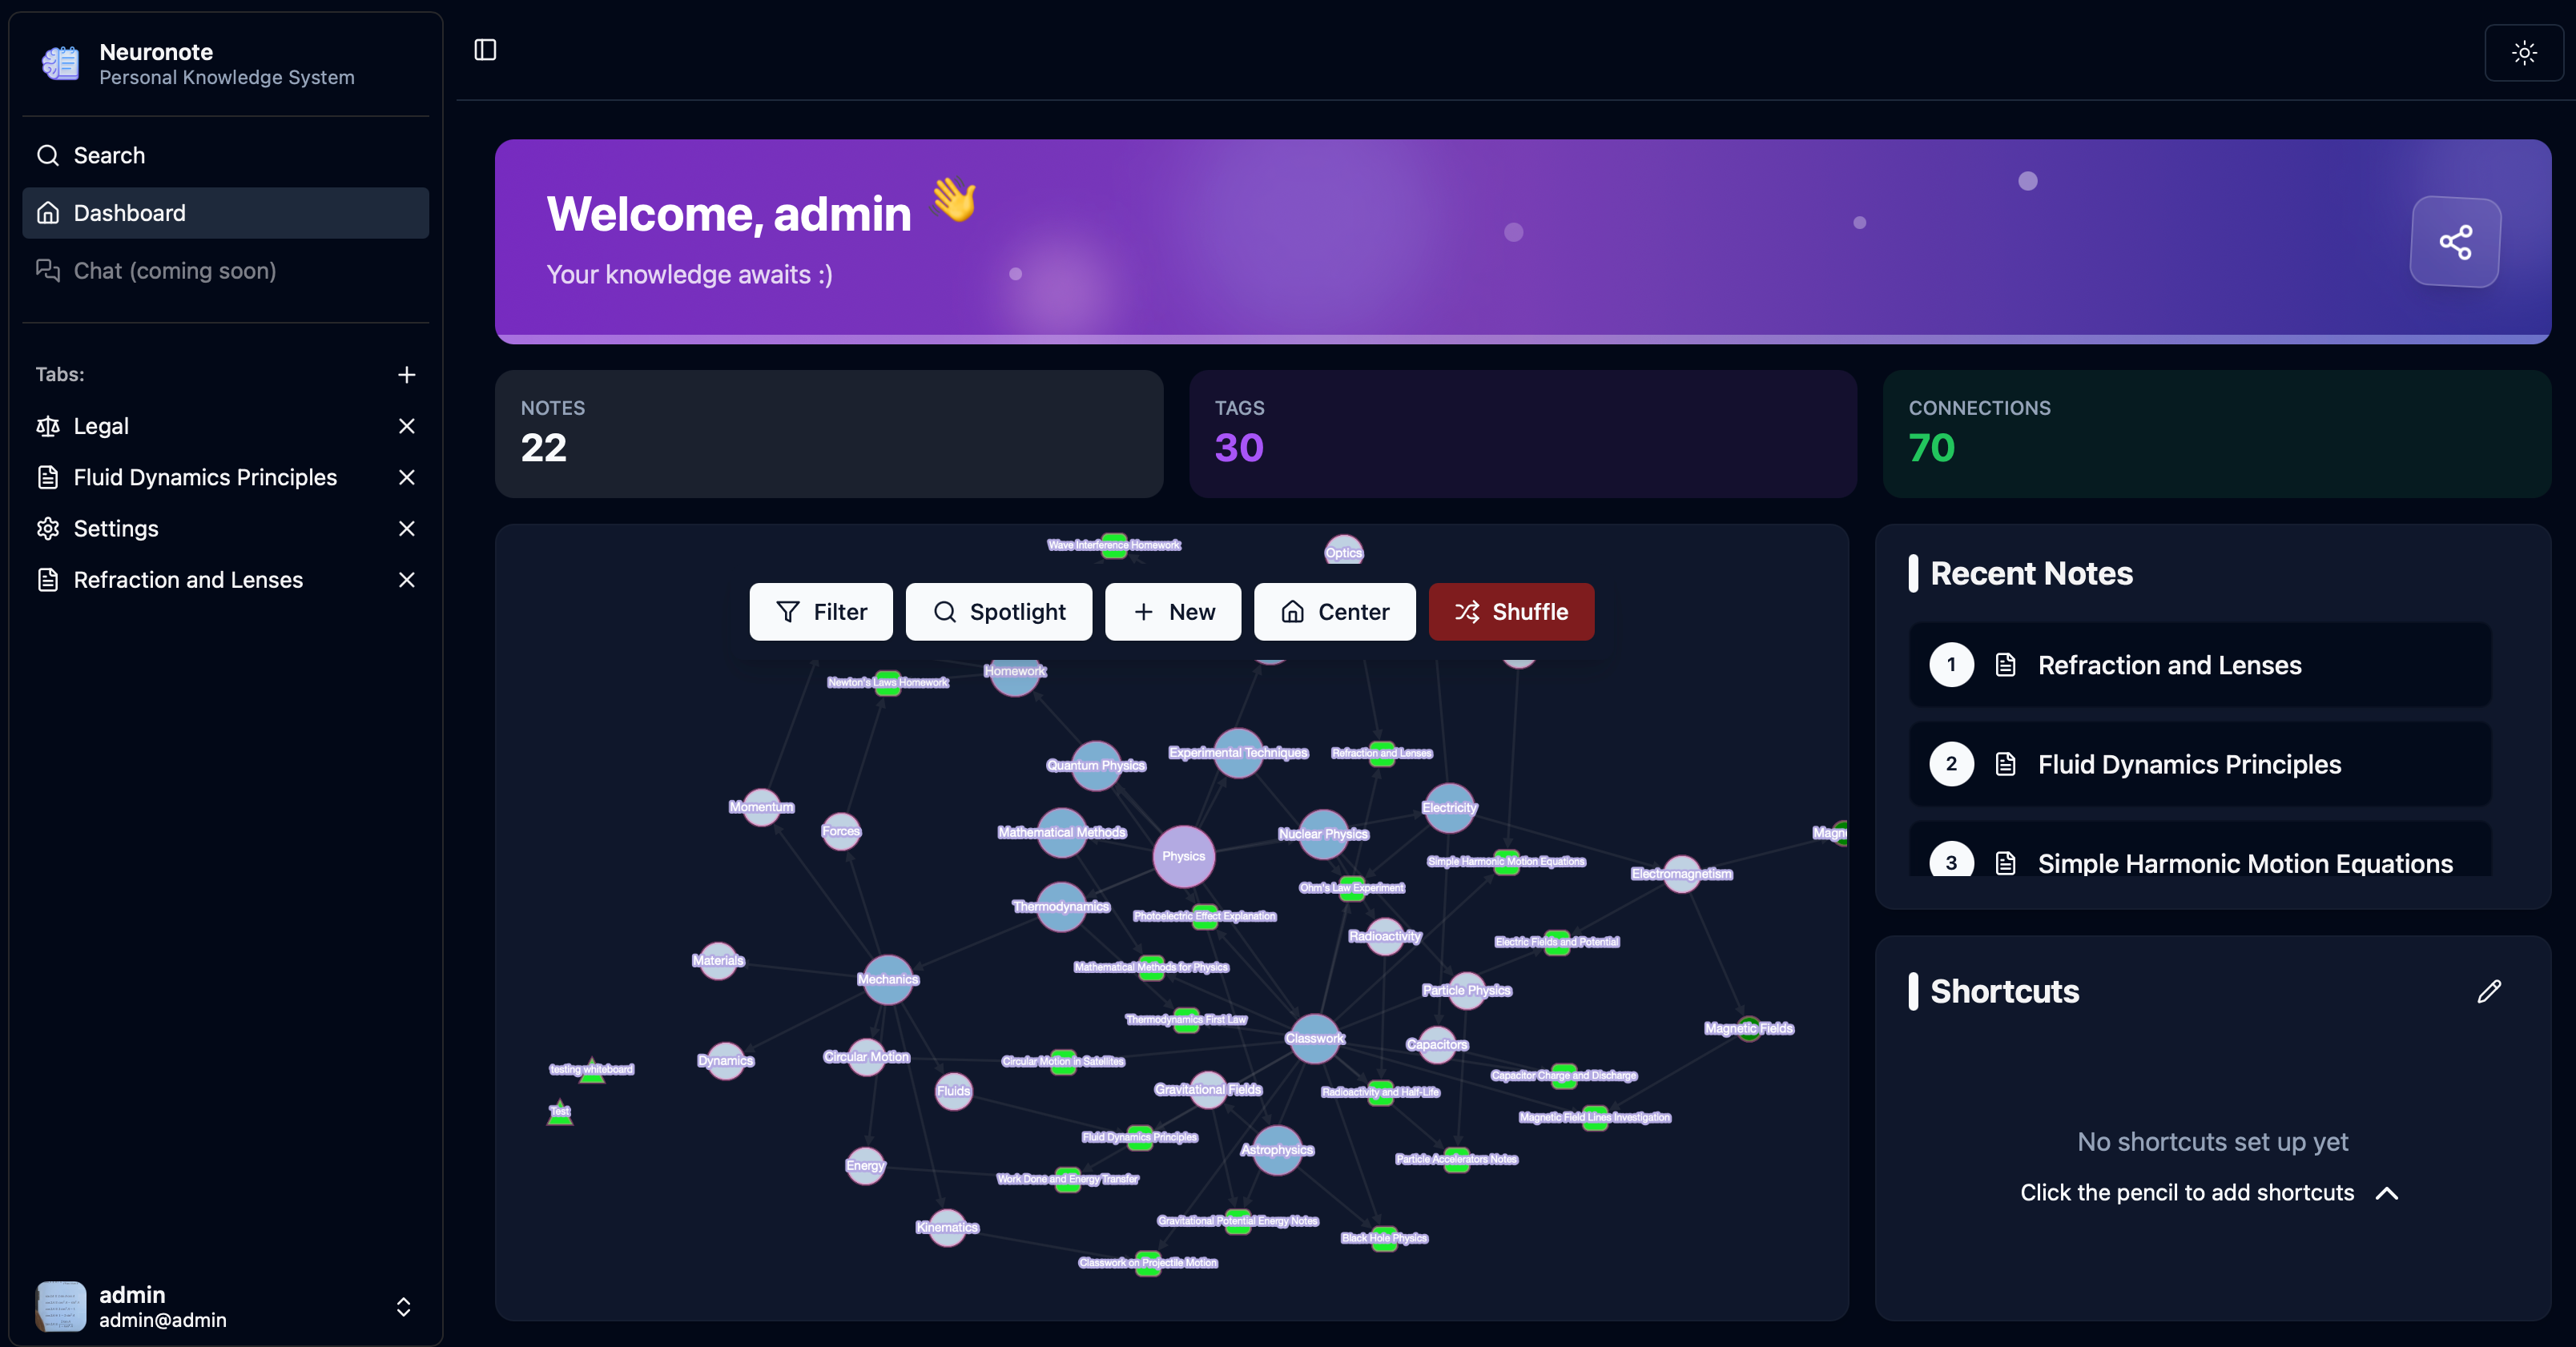
\includegraphics[width=0.8\linewidth]{Diary/27_WC_28-4-25/media/brandedPage.png}
    \caption{New branding and colour scheme}
    \label{fig:branding}
\end{figure}


\subsection*{Plans for next week:}
After Exams conclude I can't wait to jump straight back into the final couple of weeks building and completing my artifact before publicly showcasing my work for feedback
